\chapter{Labotechnieken I: veiligheid, meten en scheiden}\label{ch:b1:lab-techniques-1}

Twee studenten herkristalliseren dezelfde partij aspirine en meten het
smeltpunt op dezelfde verwarmde bank. De ene leest \qty{134}{\celsius}
af, de andere \qty{136}{\celsius}. Zijn ze het oneens? Is het product
zuiver? Geen van beide vragen kan met alleen de twee getallen beantwoord
worden: een meting is pas iets waard met haar onzekerheid, en een
vergelijking pas met een regel. Dit laatste hoofdstuk bundelt de
praktische kant van het jaar: hoe je de \omterm{def:b1:lab-techniques-1:hazard}{gevaren} leest van wat er op de
labotafel staat, hoe je een meetwaarde met haar onzekerheid opgeeft en
met een andere vergelijkt, en hoe de klassieke handelingen van het
organisch laboratorium --- extractie, filtratie, \omterm{def:b1:lab-techniques-1:recrystallisation}{herkristallisatie},
destillatie --- een product scheiden van wat het omringt, en hoe je
daarna nagaat of het zuiver is.

\begin{recall}
\omterm{def:b1:precipitation:solubility}{Oplosbaarheid} en \omterm{def:b1:intermolecular-forces-solvents:miscibility}{mengbaarheid} vanuit intermoleculaire krachten, polaire
en apolaire oplosmiddelen (\cref{ch:b1:intermolecular-forces-solvents});
buretten, pipetten en het \omterm{def:b1:titration-methods:titration}{eindpunt} van een \omterm{def:b1:titration-methods:titration}{titratie}
(\cref{ch:b1:titration-methods}). Het schoolboek (jaar 10) introduceerde
de vloeistof-vloeistofextractie, de \omterm{def:b1:lab-techniques-1:recrystallisation}{herkristallisatie}, de
dunnelaagchromatografie en het \omterm{def:b1:extent-q-and-k:fractional-extent}{rendement} van een synthese; hier krijgen
ze hun getallen.
\end{recall}

\begin{omfigure}
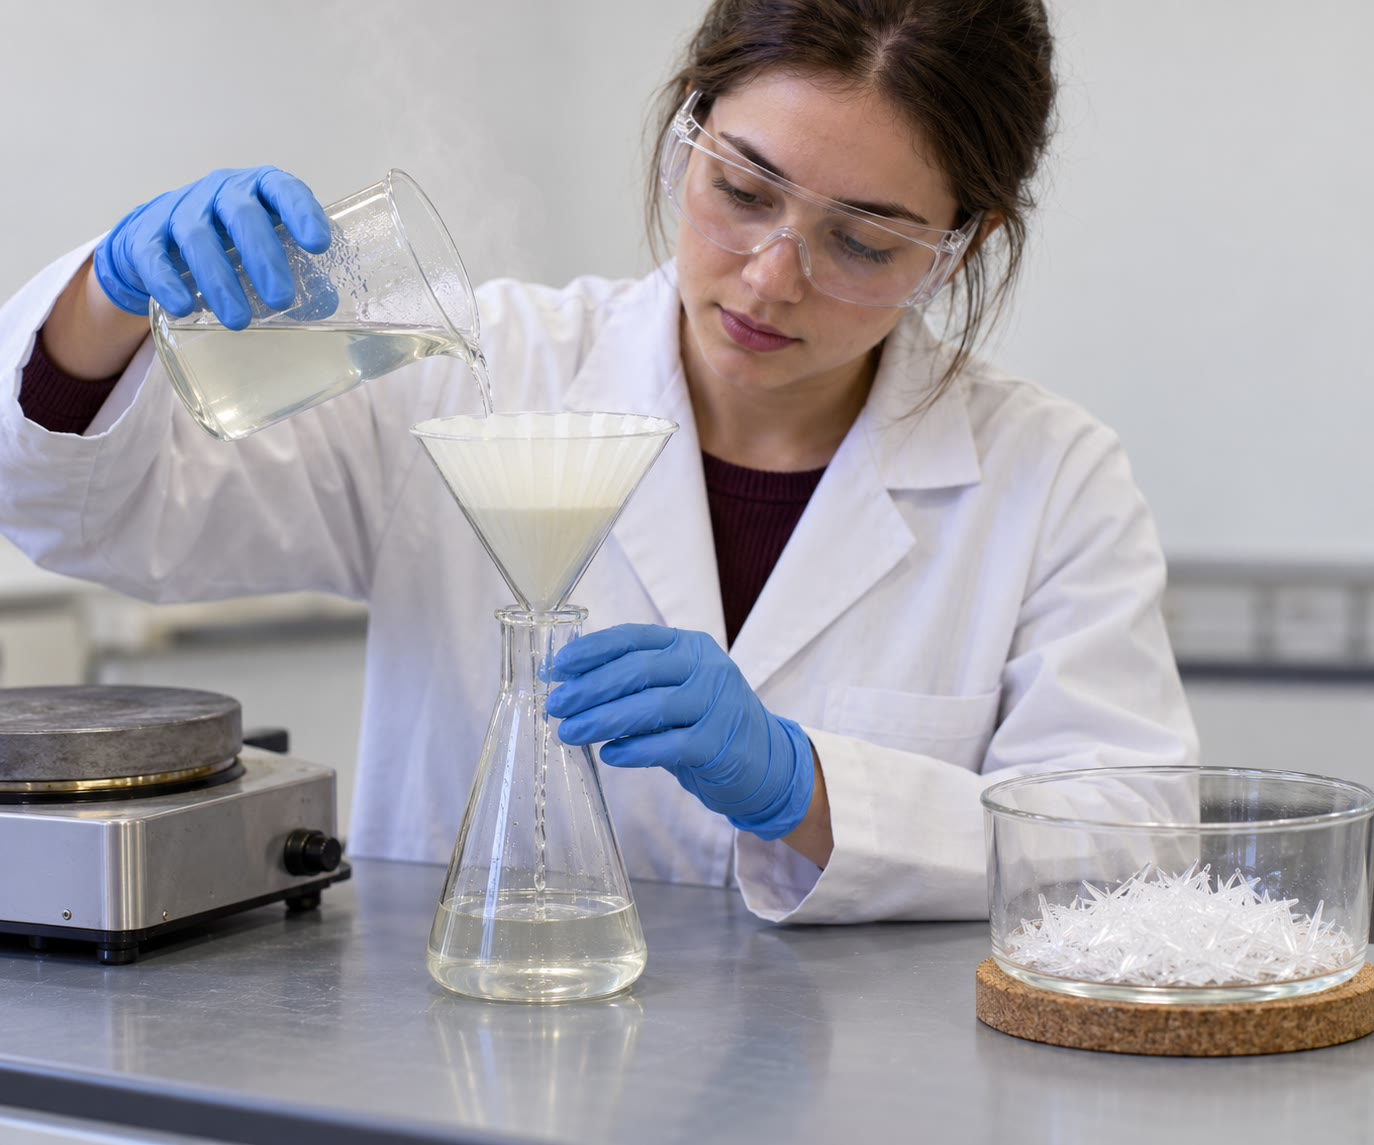
\includegraphics[width=0.5\linewidth]{images/book2/ai/b1-29-recrystallisation.jpg}

{\small Warme filtratie tijdens een \omterm{def:b1:lab-techniques-1:recrystallisation}{herkristallisatie}: veiligheidsbril,
handschoenen en labojas; de hete oplossing loopt door een plooifilter,
dat de onoplosbare onzuiverheden tegenhoudt. Naalden van een
geherkristalliseerd product wachten in het schaaltje rechts.}
\end{omfigure}

\section{Gevaren en hun etiketten}

\begin{definition}[Gevaar en risico]\label{def:b1:lab-techniques-1:hazard}
Een \emph{gevaar}\index{gevaar} is de intrinsieke eigenschap van een stof
(of van een situatie) die schade kan veroorzaken: ontvlambaarheid,
bijtendheid, giftigheid. Het \emph{risico}\index{risico} is de kans dat de
schade zich werkelijk voordoet, en de ernst ervan, onder de gegeven
gebruiksomstandigheden: het hangt af van het gevaar en van de blootstelling
(hoeveelheid, concentratie, duur, blootstellingsweg, bescherming).
\end{definition}

Een \omterm{def:b1:lab-techniques-1:hazard}{gevaar} kan niet veranderd worden zonder de stof te veranderen; een
\omterm{def:b1:lab-techniques-1:hazard}{risico} wordt verkleind door op de blootstelling in te werken: een
kleinere hoeveelheid, een meer verdunde oplossing, een zuurkast,
handschoenen en veiligheidsbril, of een minder gevaarlijk reagens voor
hetzelfde werk.

\begin{definition}[GHS-etikettering]\label{def:b1:lab-techniques-1:ghs}
De etiketten van chemicaliën volgen het Globally Harmonized System (GHS).
\begin{itemize}
  \item Een \emph{gevarenpictogram}\index{gevarenpictogram} is een zwart
        symbool op een witte ruit met een rode rand; er zijn er negen,
        \texttt{GHS01} tot \texttt{GHS09}.
  \item Het \emph{signaalwoord}\index{signaalwoord} is \emph{Gevaar} voor
        de ernstigere gevarencategorieën en \emph{Waarschuwing} voor de
        minder ernstige; een etiket draagt er maar één, het ernstigste.
  \item Een \emph{gevarenaanduiding}\index{gevarenaanduiding} is een
        standaardzin, gecodeerd met H gevolgd door drie cijfers, die een
        \omterm{def:b1:lab-techniques-1:hazard}{gevaar} beschrijft: H2xx fysische \omterm{def:b1:lab-techniques-1:hazard}{gevaren}, H3xx \omterm{def:b1:lab-techniques-1:hazard}{gevaren} voor de
        gezondheid, H4xx \omterm{def:b1:lab-techniques-1:hazard}{gevaren} voor het milieu.
  \item Een \emph{voorzorgsmaatregel}\index{voorzorgsmaatregel},
        gecodeerd met P en drie cijfers, geeft een te nemen maatregel:
        P1xx algemeen, P2xx preventie, P3xx reactie, P4xx opslag, P5xx
        verwijdering.
  \item Het \emph{veiligheidsinformatieblad}\index{veiligheidsinformatieblad}
        is het document dat de leverancier bij een product verstrekt, in
        standaardrubrieken: identificatie, \omterm{def:b1:lab-techniques-1:hazard}{gevaren}, samenstelling, eerste
        hulp, brandbestrijding, hantering en opslag, blootstellingscontrole
        en bescherming, fysische en chemische eigenschappen, stabiliteit,
        toxiciteit, verwijdering en transport.
\end{itemize}
\end{definition}

\begin{omfigure}
\setlength{\tabcolsep}{5pt}
\begin{tabular}{ccccc}
\begin{tabular}[t]{@{}c@{}}\ghs[1.25cm]{GHS01}\\[2pt]\footnotesize GHS01\\\footnotesize explosief\end{tabular} &
\begin{tabular}[t]{@{}c@{}}\ghs[1.25cm]{GHS02}\\[2pt]\footnotesize GHS02\\\footnotesize ontvlambaar\end{tabular} &
\begin{tabular}[t]{@{}c@{}}\ghs[1.25cm]{GHS03}\\[2pt]\footnotesize GHS03\\\footnotesize oxiderend\end{tabular} &
\begin{tabular}[t]{@{}c@{}}\ghs[1.25cm]{GHS04}\\[2pt]\footnotesize GHS04\\\footnotesize gas onder druk\end{tabular} &
\begin{tabular}[t]{@{}c@{}}\ghs[1.25cm]{GHS05}\\[2pt]\footnotesize GHS05\\\footnotesize bijtend\end{tabular} \\[8pt]
\begin{tabular}[t]{@{}c@{}}\ghs[1.25cm]{GHS06}\\[2pt]\footnotesize GHS06\\\footnotesize acute toxiciteit\end{tabular} &
\begin{tabular}[t]{@{}c@{}}\ghs[1.25cm]{GHS07}\\[2pt]\footnotesize GHS07\\\footnotesize schadelijk, irriterend\end{tabular} &
\begin{tabular}[t]{@{}c@{}}\ghs[1.25cm]{GHS08}\\[2pt]\footnotesize GHS08\\\footnotesize gezondheidsgevaar\end{tabular} &
\begin{tabular}[t]{@{}c@{}}\ghs[1.25cm]{GHS09}\\[2pt]\footnotesize GHS09\\\footnotesize milieu\end{tabular} & \\
\end{tabular}

\smallskip
{\small De negen GHS-pictogrammen: ontploffende bom, vlam, vlam boven een
cirkel, gasfles, corrosie, doodshoofd met gekruiste beenderen,
uitroepteken, gezondheidsgevaar (effecten op lange termijn: kanker,
mutaties, voortplanting, sensibilisatie van de luchtwegen, aspiratie) en
milieu.}
% ledger: ghspic:GHS01, ghspic:GHS02, ghspic:GHS03, ghspic:GHS04,
% ghspic:GHS05, ghspic:GHS06, ghspic:GHS07, ghspic:GHS08, ghspic:GHS09
\end{omfigure}

\begin{example}[Het etiket van ethanol lezen]
Een fles ethanol draagt de pictogrammen GHS02 en GHS07, het \omterm{def:b1:lab-techniques-1:ghs}{signaalwoord}
\emph{Gevaar}, en de aanduidingen H225 (licht ontvlambare vloeistof en
damp, een fysisch \omterm{def:b1:lab-techniques-1:hazard}{gevaar}, waarvan de categorie \emph{Gevaar} vereist) en
H319 (veroorzaakt ernstige oogirritatie, een \omterm{def:b1:lab-techniques-1:hazard}{gevaar} voor de gezondheid,
op zich \emph{Waarschuwing}). Tot de \omterm{def:b1:lab-techniques-1:ghs}{voorzorgsmaatregelen} behoren P210
(verwijderd houden van warmte, vonken en open vuur; niet roken), P233 (in
goed gesloten verpakking bewaren), P280 (handschoenen en oogbescherming
dragen), P305+P351+P338 (bij contact met de ogen: voorzichtig gedurende
een aantal minuten met water afspoelen, contactlenzen verwijderen, blijven
spoelen) en P403+P235 (op een goed geventileerde plaats bewaren, koel
bewaren). De praktische gevolgen: geen vlam op de labotafel waar ethanol
gebruikt wordt, een veiligheidsbril, een gesloten fles.
\end{example}
% ledger: ghs:ethanol, hstat:H225, hstat:H319, pstat:P210, pstat:P233,
% pstat:P280, pstat:P305+P351+P338, pstat:P403+P235

\begin{method}[Een practicum voorbereiden met de veiligheidsinformatiebladen]\label{met:b1:lab-techniques-1:read-sds}
Voor elke stof die gebruikt of gevormd wordt:
\begin{enumerate}
  \item lees haar pictogrammen, \omterm{def:b1:lab-techniques-1:ghs}{signaalwoord} en H-zinnen (rubriek 2 van
        het blad), en noteer de fysische \omterm{def:b1:lab-techniques-1:hazard}{gevaren} (brand, druk,
        reactiviteit) apart van die voor de gezondheid en het milieu;
  \item schat voor elke handeling (wegen, verwarmen, overbrengen,
        filtreren) de blootstelling in: hoeveelheid, toestand (een
        vluchtige vloeistof of een fijn poeder bereikt de longen), duur;
  \item kies de maatregelen: vervanging door een minder gevaarlijk
        reagens, een kleinere schaal, een zuurkast, daarna persoonlijke
        bescherming (P2xx-zinnen);
  \item plan de reactie op een incident (P3xx: ogen, huid, inslikken,
        brand) en waar elk afval naartoe gaat (P5xx).
\end{enumerate}
\end{method}

\begin{inthelab}[Afval]
Niets gaat standaard door de gootsteen. Organische oplosmiddelen worden
in twee recipiënten verzameld, gehalogeneerd (dichloormethaan,
chloroform) en niet-gehalogeneerd (ethanol, propanon, cyclohexaan,
ethylethanoaat), omdat ze verschillend verwerkt worden; waterige zure en
basische oplossingen worden geneutraliseerd voordat ze afgevoerd worden;
oplossingen van zwaremetaalionen (chroom, koper, zilver) hebben hun eigen
recipiënten; glasscherven en verontreinigde vaste stoffen worden apart
gehouden van gewoon huisvuil. De zin P273, ``voorkomen dat het product in
het milieu terechtkomt'', op een etiket herinnert eraan dat het
afvalrecipiënt, en niet de afvoer, het eindpunt van het experiment is.
% ledger: pstat:P273
\end{inthelab}

\section{Meten en onzekerheid}

Een meetwaarde is nooit de exacte waarde van de gemeten grootheid: herhaal
de meting en het resultaat verandert een beetje; lees de schaal af en het
laatste cijfer is een schatting. De onzekerheid zegt hoe ver van de
meetwaarde de ware waarde redelijkerwijs kan liggen.

\begin{definition}[Meetonzekerheid]\label{def:b1:lab-techniques-1:uncertainty}
\begin{itemize}
  \item De \emph{meetonzekerheid}\index{meetonzekerheid} is een parameter
        die de spreiding kenmerkt van de waarden die redelijkerwijs aan de
        gemeten grootheid toegekend kunnen worden.
  \item De \emph{standaardonzekerheid}\index{standaardonzekerheid} $u(x)$
        is die onzekerheid uitgedrukt als een standaardafwijking.
  \item Een \emph{type-A-evaluatie}\index{type-A-evaluatie} verkrijgt $u$
        door de statistische analyse van een reeks herhaalde metingen; een
        \emph{type-B-evaluatie}\index{type-B-evaluatie} verkrijgt haar op
        elke andere manier: de schaalverdeling van een instrument, de
        tolerantie die de fabrikant opgeeft, een kalibratiecertificaat,
        het aantal cijfers van een getabelleerde waarde.
  \item De \emph{uitgebreide onzekerheid}\index{uitgebreide onzekerheid}
        $U = k\,u$ is de standaardonzekerheid vermenigvuldigd met een
        dekkingsfactor $k$, meestal $k = 2$; voor een normale verdeling
        bevat het interval $x \pm 2u$ de ware waarde met een kans van
        ongeveer \qty{95}{\percent}.
  \item De \emph{relatieve onzekerheid}\index{relatieve onzekerheid} is
        $u(x)/|x|$, vaak in procent opgegeven.
\end{itemize}
\end{definition}

\begin{proposition}[Type-A-evaluatie]\label{prop:b1:lab-techniques-1:type-a}
Als er $n$ onafhankelijke metingen $x_1, \dots, x_n$ van dezelfde grootheid
uitgevoerd worden, is hun gemiddelde $\bar x$ de beste schatting; de
experimentele standaardafwijking is
\[
  s = \sqrt{\frac{1}{n-1} \sum_{i=1}^{n} (x_i - \bar x)^2},
\]
en de \omterm{def:b1:lab-techniques-1:uncertainty}{standaardonzekerheid} van het gemiddelde is $u(\bar x) = s/\sqrt{n}$.
\end{proposition}
\begin{proof}[\omnameProof]
\emph{Op dit niveau aangenomen}; de statistiek van herhaalde metingen,
met inbegrip van de studentcoëfficiënt die gebruikt wordt wanneer $n$
klein is, wordt in het deel van jaar 2 behandeld.
\end{proof}

\begin{omfigure}
\begin{tikzpicture}
\begin{axis}[width=7.4cm, height=5cm, xlabel={eindpuntvolume (\unit{mL})},
  ylabel={aantal aflezingen}, ymin=0, ymax=8.5, xmin=12.2, xmax=12.7,
  xtick={12.2,12.3,12.4,12.5,12.6,12.7},
  xticklabel style={/pgf/number format/fixed, /pgf/number format/precision=1},
  axis lines=left, every axis plot/.append style={line join=round}]
  \addplot[ybar, bar width=0.045, fill=omDef!35, draw=omDef!80!black]
    table[x=V, y=count] {figdata/out/bachelor-1-type-a-uncertainty-a.dat};
  \addplot[omThm, thick, smooth]
    table[x=V, y=g] {figdata/out/bachelor-1-type-a-uncertainty-b.dat};
  \draw[omProp, thick, <->] (axis cs:12.384,7.6) -- (axis cs:12.526,7.6);
  \node[omProp, font=\small, above] at (axis cs:12.455,7.6) {$\bar V \pm s$};
\end{axis}
\end{tikzpicture}\hspace{0.6cm}%
\begin{tikzpicture}
\begin{axis}[width=5.6cm, height=5cm, xlabel={$x - x_0$}, ylabel={dichtheid},
  ymin=0, ymax=0.8, xmin=-1.6, xmax=1.6, xtick={-1,0,1},
  xticklabels={$-a$, $0$, $a$}, ytick={0.5}, yticklabels={$\frac{1}{2a}$},
  axis lines=left]
  \addplot[omDef!80!black, thick, fill=omDef!25] coordinates
    {(-1,0) (-1,0.5) (1,0.5) (1,0)} \closedcycle;
  \draw[omProp, thick, <->] (axis cs:-0.577,0.62) -- (axis cs:0.577,0.62);
  \node[omProp, font=\small, above] at (axis cs:0,0.62) {$\pm a/\sqrt3$};
\end{axis}
\end{tikzpicture}

{\small Links: twintig aflezingen van hetzelfde \omterm{def:b1:titration-methods:titration}{eindpunt} van een \omterm{def:b1:titration-methods:titration}{titratie}
(illustratieve gegevens), afgelezen tot op \qty{0.05}{mL}, met de normale
kromme met hetzelfde gemiddelde $\bar V = \qty{12.455}{mL}$ en dezelfde
standaardafwijking $s = \qty{0.071}{mL}$. Rechts: de rechthoekige verdeling
van een \omterm{def:b1:lab-techniques-1:uncertainty}{type-B-evaluatie}, een waarde waarvan alleen bekend is dat ze
tussen $x_0 - a$ en $x_0 + a$ ligt; haar standaardafwijking is
$a/\sqrt3$.}
\end{omfigure}

\begin{example}[Twintig eindpunten]
Voor de twintig aflezingen van de figuur is $\bar V = \qty{12.455}{mL}$,
$s = \qty{0.071}{mL}$ en $u(\bar V) = 0.071/\sqrt{20} = \qty{0.016}{mL}$.
Eén aflezing is onzeker tot op ongeveer $s$; het gemiddelde van twintig
tot op ongeveer $s/\sqrt{20}$, vierenhalve keer minder. Het resultaat is
$V = \qty{12.46}{mL}$ met $U = 2u = \qty{0.03}{mL}$.
\end{example}

\begin{proposition}[Type-B-evaluatie voor een rechthoekige verdeling]\label{prop:b1:lab-techniques-1:type-b}
Als het enige wat over een grootheid bekend is, is dat ze met gelijke
waarschijnlijkheid ergens tussen $x_0 - a$ en $x_0 + a$ ligt, dan is haar
\omterm{def:b1:lab-techniques-1:uncertainty}{standaardonzekerheid}
\[
  u = \frac{a}{\sqrt3}.
\]
\end{proposition}
\begin{proof}
De kansdichtheid is $1/(2a)$ op $[x_0 - a, x_0 + a]$ en elders nul; haar
gemiddelde is $x_0$ wegens de symmetrie en haar variantie is
\[
  u^2 = \int_{x_0-a}^{x_0+a} (x - x_0)^2 \frac{\mathrm{d}x}{2a}
      = \frac{1}{2a} \left[\frac{t^3}{3}\right]_{-a}^{a}
      = \frac{1}{2a}\cdot\frac{2a^3}{3} = \frac{a^2}{3}. \qedhere
\]
\end{proof}

\begin{example}[Een aflezing en een tolerantie]
Een buret met een schaalverdeling om de \qty{0.1}{mL} wordt tot op een
half schaaldeel afgelezen: de aflezing ligt binnen $\pm\qty{0.05}{mL}$
van de genoteerde waarde, dus $u = 0.05/\sqrt3 = \qty{0.029}{mL}$. Een
pipet van \qty{20}{mL} waarvoor de fabrikant een tolerantie van
$\pm\qty{0.03}{mL}$ opgeeft, levert haar volume met
$u = 0.03/\sqrt3 = \qty{0.017}{mL}$. Een getabelleerde waarde die als
\qty{135}{\celsius} gegeven wordt, is bekend tot op
$\pm\qty{0.5}{\celsius}$: $u = \qty{0.29}{\celsius}$.
\end{example}

\begin{proposition}[Onzekerheden combineren]\label{prop:b1:lab-techniques-1:combine}
Voor onafhankelijke grootheden: als $y = x_1 + x_2$ of $y = x_1 - x_2$, dan
is $u(y)^2 = u(x_1)^2 + u(x_2)^2$; als $y = x_1 x_2$ of $y = x_1/x_2$, dan
\[
  \left(\frac{u(y)}{y}\right)^2 = \left(\frac{u(x_1)}{x_1}\right)^2
  + \left(\frac{u(x_2)}{x_2}\right)^2 .
\]
Meerdere bronnen van onzekerheid op dezelfde grootheid (een type-A-deel en
type-B-delen) combineren op dezelfde manier, als een som van kwadraten.
\end{proposition}
\admitted

De kwadraten, niet de onzekerheden zelf, worden opgeteld: twee
onafhankelijke fouten duwen zelden met volle grootte in dezelfde
richting. Een getitreerd volume is een verschil van twee
buretaflezingen, dus zijn afleesonzekerheid is
$\sqrt2 \times \qty{0.029}{mL} = \qty{0.041}{mL}$; en één grote bron van
onzekerheid overheerst de andere, en daar moet een verbetering gezocht
worden. De algemene regel, met partiële afgeleiden, hoort bij het deel van
jaar 2.

\begin{method}[Een resultaat rapporteren]\label{met:b1:lab-techniques-1:report-result}
\begin{enumerate}
  \item Som de bronnen van onzekerheid op; evalueer elk ervan als een
        \omterm{def:b1:lab-techniques-1:uncertainty}{standaardonzekerheid} (type A uit een reeks, type B als $a/\sqrt3$
        uit een halve breedte).
  \item Combineer ze als een som van kwadraten (\cref{prop:b1:lab-techniques-1:combine}).
  \item Geef de \omterm{def:b1:lab-techniques-1:uncertainty}{uitgebreide onzekerheid} $U = 2u$ met één of twee
        beduidende cijfers, en rond de waarde af op dezelfde decimaal:
        $x = (\text{waarde} \pm U)$ eenheid, $k = 2$.
\end{enumerate}
\end{method}

\begin{definition}[Genormaliseerde afwijking]\label{def:b1:lab-techniques-1:z-score}
De \emph{genormaliseerde afwijking}\index{genormaliseerde afwijking} (of
$z$-score) tussen twee onafhankelijke waarden $x_1$ en $x_2$ van dezelfde
grootheid, met standaardonzekerheden $u_1$ en $u_2$, is
\[
  z = \frac{|x_1 - x_2|}{\sqrt{u_1^2 + u_2^2}} .
\]
De twee waarden heten compatibel wanneer $z \le 2$; een meetwaarde is
onder dezelfde voorwaarde compatibel met een referentiewaarde.
\end{definition}

\begin{example}[De twee studenten]
De twee smeltpunten van de inleiding, \qty{134}{\celsius} en
\qty{136}{\celsius}, werden elk verkregen met een \omterm{def:b1:lab-techniques-1:uncertainty}{standaardonzekerheid}
van \qty{0.8}{\celsius} (aflezing en kalibratie van de bank). Dan is
$z = 2/\sqrt{0.8^2 + 0.8^2} = 1.8 \le 2$: de studenten zijn het eens. Hun
gemiddelde, \qty{135}{\celsius}, is ook compatibel met het getabelleerde
smeltpunt van aspirine, \qty{135}{\celsius} bij snelle verwarming. Een
getabelleerde waarde die tot op de eenheid gegeven wordt, heeft
$u = 0.5/\sqrt3 = \qty{0.29}{\celsius}$, zodat één aflezing met
$u = \qty{0.8}{\celsius}$ ermee compatibel is zolang ze binnen
$2\sqrt{0.8^2 + 0.29^2} = \qty{1.7}{\celsius}$ ervan ligt: een aflezing
onder ongeveer \qty{133}{\celsius} zou op een onzuiver product gewezen
hebben.
\end{example}
% ledger: mp:aspirin

% Keep the heading with the definition box below it: break here if fewer
% than about eight lines are left, otherwise the two glues cancel.
\par\vspace{0pt plus 8\baselineskip}\penalty-200\vspace{0pt plus -8\baselineskip}
\section{Scheiden}

\begin{definition}[Verdelingscoëfficiënt]\label{def:b1:lab-techniques-1:partition-coefficient}
Wanneer een opgeloste stof A bij evenwicht verdeeld is over twee niet
mengbare oplosmiddelen, een organische \omterm{def:b1:extent-q-and-k:system}{fase} en een waterfase, is de
verhouding van haar concentraties
\[
  K = \frac{[\mathrm{A}]_{\mathrm{org}}}{[\mathrm{A}]_{\mathrm{aq}}}
\]
voor verdunde oplossingen bij een gegeven temperatuur een constante: de
\emph{verdelingscoëfficiënt}\index{verdelingscoefficient@verdelingscoëfficiënt} van A tussen de
twee oplosmiddelen.
\end{definition}

\begin{proposition}[Meerdere extracties zijn beter dan één]\label{prop:b1:lab-techniques-1:multiple-extractions}
Een volume $V_a$ waterige oplossing wordt $n$ keer geëxtraheerd, telkens
met een vers volume $V_o$ organisch oplosmiddel. De fractie A die in de
waterfase achterblijft, is
\[
  f_n = \left(1 + K \frac{V_o}{V_a}\right)^{-n}.
\]
Voor een vast totaalvolume oplosmiddel extraheren $n$ kleine porties meer
dan één grote portie.
\end{proposition}
\begin{proof}
Zij $m$ de hoeveelheid A in de waterfase vóór een extractie, en $m'$
erna. Bij evenwicht bevat de organische \omterm{def:b1:extent-q-and-k:system}{fase} $m - m'$, en
$K = \dfrac{(m - m')/V_o}{m'/V_a}$, dus $m - m' = K\dfrac{V_o}{V_a} m'$ en
$m' = m\big/\bigl(1 + K V_o/V_a\bigr)$. Elke extractie vermenigvuldigt de
overblijvende hoeveelheid met dezelfde factor; na $n$ extracties is $f_n$
de $n$-de macht. Met een totaalvolume $V$ verdeeld in $n$ porties $V/n$ is
$\ln f_n = -n \ln(1 + KV/(nV_a))$; omdat $\ln(1+t)/t$ daalt met $t$,
stijgt $n \ln(1 + t/n)$ met $n$ voor $t = KV/V_a > 0$, en daalt $f_n$, naar
de limiet $\mathrm{e}^{-KV/V_a}$.
\end{proof}

\begin{example}[Eén portie of drie]
Een opgeloste stof met $K = 4$ wordt uit \qty{100}{mL} water geëxtraheerd
met \qty{60}{mL} ethylethanoaat. In één portie is
$f_1 = 1/(1 + 4 \times 0.6) = 0.29$: \qty{71}{\percent} wordt
geëxtraheerd. In drie porties van \qty{20}{mL} is
$f_3 = (1 + 4 \times 0.2)^{-3} = 0.17$: \qty{83}{\percent}.
Ethylethanoaat ($\rho = \qty{0.90}{g/cm^3}$) is de bovenste laag in de
scheitrechter; dichloormethaan ($\rho = \qty{1.33}{g/cm^3}$) zou de
onderste zijn.
\end{example}
% ledger: rho:ethyl-acetate, rho:CH2Cl2, rho:water

Filtratie scheidt een vaste stof van een vloeistof. Door de zwaartekracht,
door een plooifilter in een trechter, houdt ze een onoplosbare
onzuiverheid tegen uit een hete oplossing die onderweg niet mag afkoelen
(warme filtratie, zoals op de foto aan het begin van het hoofdstuk). Onder
verminderde druk, in een büchnertrechter op een afzuigkolf (zoals
getekend in het schoolboek), verzamelt ze een vaste stof snel en laat ze
die bijna droog achter; de vaste stof wordt op de filter gewassen met een
beetje koud oplosmiddel.

\begin{definition}[Herkristallisatie]\label{def:b1:lab-techniques-1:recrystallisation}
De \emph{herkristallisatie}\index{herkristallisatie} zuivert een vaste stof
door ze op te lossen in een minimum aan heet oplosmiddel waarin ze warm
zeer goed en koud weinig oplosbaar is, en ze daarna bij het afkoelen te
laten kristalliseren; de onzuiverheden blijven ofwel opgelost in het koude
oplosmiddel (de moederloog), ofwel worden ze, als ze onoplosbaar zijn,
vooraf door warme filtratie verwijderd.
\end{definition}

\begin{method}[Een vaste stof herkristalliseren]\label{met:b1:lab-techniques-1:recrystallise}
\begin{enumerate}
  \item Kies het oplosmiddel: het product warm zeer goed en koud weinig
        oplosbaar, de oplosbare onzuiverheden ook koud oplosbaar, geen
        reactie met het product, een kookpunt onder het smeltpunt van het
        product; een mengsel van twee \omterm{def:b1:intermolecular-forces-solvents:miscibility}{mengbare} oplosmiddelen (ethanol en
        water) kan op het product afgestemd worden.
  \item Los de ruwe vaste stof op in het minimum aan kokend oplosmiddel,
        in kleine porties toegevoegd, onder reflux als het oplosmiddel
        vluchtig of ontvlambaar is.
  \item Blijft er een onoplosbare onzuiverheid over, filtreer dan warm.
  \item Laat de oplossing langzaam afkoelen, daarna in ijs: langzaam
        afkoelen geeft grotere, zuiverdere \omterm{def:b1:crystals-metals:crystal}{kristallen}, die minder
        moederloog insluiten.
  \item Filtreer onder verminderde druk, was met een beetje ijskoud
        oplosmiddel, droog, weeg; controleer de zuiverheid (smeltpunt,
        DLC).
\end{enumerate}
\end{method}

\begin{example}[De prijs van zuiverheid]
Aspirine lost in water op tot ongeveer \qty{3.3}{g/L} bij
\qty{25}{\celsius} en \qty{10}{g/L} bij \qty{37}{\celsius}, veel meer
dicht bij het kookpunt. Als \qty{40}{mL} moederloog en \qty{10}{mL}
waswater de filter bij \qty{25}{\celsius} verlaten, voeren ze ongeveer
$\qty{0.050}{L} \times \qty{3.3}{g/L} = \qty{0.17}{g}$ aspirine mee, ongeacht
haar zuiverheid. Elke milliliter oplosmiddel boven het minimum
kost \omterm{def:b1:extent-q-and-k:fractional-extent}{rendement}.
\end{example}
% ledger: sol:aspirin-25, sol:aspirin-37

Een vloeistof wordt gezuiverd, of twee vloeistoffen met ver uit elkaar
liggende kookpunten worden gescheiden, door \emph{enkelvoudige
destillatie}: het mengsel wordt aan de kook gebracht, en de damp, rijker
aan de vluchtigste component, wordt gecondenseerd en opgevangen. De
temperatuur aan de zijarm is die van de damp die overdestilleert; zolang
ze constant blijft, gaat er een zuivere stof over. Vloeistoffen met dicht
bij elkaar liggende kookpunten vragen een gefractioneerde destillatie,
met een kolom tussen de kolf en de destillatiekop, die met de
vloeistof-dampdiagrammen van het deel van jaar 2 behandeld wordt.

\begin{omfigure}
\begin{tikzpicture}[font=\small, scale=0.95]
  \pic[transform shape] at (0,0) {heatingmantle};
  \pic[transform shape] at (0,0) {rbflask={0.45}{orange!25}};
  \foreach \x/\y in {-0.35/0.25,0.05/0.18,0.35/0.3}
    \fill[black!55] (\x,\y) circle (0.06);
  \pic[transform shape] (s) at (0,3.0) {stillhead};
  \pic[transform shape] at ($(s-top)+(0,-0.75)$) {thermometer};
  \pic[transform shape, rotate=-20] (c) at (s-arm) {liebig={3.4}};
  \coordinate (cend) at ($(s-arm)+(-20:3.4)$);
  \pic[transform shape] (a) at (cend) {adapter};
  \pic[transform shape] at ($(a-tip)+(0,-2.4)$) {erlenmeyer={0.22}{orange!12}};
  \draw[<-, omProp, thick] (0.12,3.72) -- (-1.4,4.4) node[left, text=black,
    align=right] {thermometerreservoir\\ ter hoogte van de zijarm};
  \draw[<-, omProp, thick] ($(s-arm)+(-20:0.65)+(0.65,0.65)$) -- ++(0.2,0.9)
    node[above, text=black] {water uit};
  \draw[<-, omProp, thick] ($(s-arm)+(-20:2.7)+(-0.2,-0.6)$) -- ++(0.05,-0.9)
    node[below, text=black] {water in};
  \draw[<-, omProp, thick] (-0.3,0.27) -- (-2.2,0.7) node[left, text=black]
    {kooksteentjes};
  \draw[<-, omProp, thick] (1.35,-0.6) -- (2.3,-1.1) node[right, text=black]
    {verwarmingsmantel};
  \draw[<-, omProp, thick] ($(a-tip)+(0.75,-2.0)$) -- ++(1.0,0.2)
    node[right, text=black] {destillaat};
\end{tikzpicture}

{\small Enkelvoudige destillatie. De thermometer meet de temperatuur van
de damp die de koeler binnenkomt; het koelwater komt aan het lage uiteinde
van de koeler binnen, zodat de mantel vol blijft; de kooksteentjes
voorkomen heftig stoten; de opstelling staat bij de opvangkolf in
verbinding met de lucht.}
\end{omfigure}

\begin{safety}{\ghs[5mm]{GHS02}}
Een destillatieopstelling is nooit gesloten: een afgesloten systeem dat
verwarmd wordt, barst. Kooksteentjes worden aan de koude vloeistof
toegevoegd, nooit aan een vloeistof die al heet is (die kan meteen
overkoken). Een ontvlambaar destillaat wordt ver van elke vlam
opgevangen, de opvangkolf zo nodig in ijs.
\end{safety}

\section{Identificeren en de zuiverheid controleren}

\begin{definition}[Retentiefactor]\label{def:b1:lab-techniques-1:retention-factor}
Bij dunnelaagchromatografie (DLC) wordt een vlek van het monster
aangebracht op een startlijn dicht bij de onderkant van een plaat die met
een stationaire \omterm{def:b1:extent-q-and-k:system}{fase} (silica) bedekt is; de plaat staat in een gesloten
tank in een beetje eluens, dat door capillariteit door de laag omhoog
trekt en de deeltjes met verschillende snelheden meevoert. De
\emph{retentiefactor}\index{retentiefactor} van een deeltje is
\[
  R_f = \frac{\text{afstand afgelegd door de vlek}}
             {\text{afstand afgelegd door het eluensfront}},
\]
beide gemeten vanaf de startlijn; $0 \le R_f \le 1$, en bij een gegeven
stationaire \omterm{def:b1:extent-q-and-k:system}{fase}, eluens en temperatuur kenmerkt hij het deeltje.
\end{definition}

Op polaire silica wordt een polair deeltje sterker tegengehouden dan een
minder polair en heeft het de kleinere $R_f$; een polairder eluens
verplaatst elke vlek verder. Twee deeltjes met dezelfde $R_f$ op één
plaat kunnen toch verschillen; twee verschillende $R_f$-waarden bewijzen
dat ze verschillen. Een zuiver product geeft één enkele vlek.

\begin{omfigure}
\begin{tikzpicture}[font=\small, scale=1.7]
  \pic[transform shape] at (0,0) {tlcplate};
  \draw[omDef!80!black, densely dashed, line width=0.5pt] (-0.7,2.7) -- (0.7,2.7);
  \foreach \x in {-0.4,0,0.4} \fill[black!60] (\x,0.4) circle (0.025);
  \fill[omThm!70] (-0.4,{0.4+0.30*2.3}) ellipse (0.09 and 0.06);
  \fill[omDef!70] (0,{0.4+0.65*2.3}) ellipse (0.09 and 0.06);
  \fill[omThm!70] (0.4,{0.4+0.30*2.3}) ellipse (0.09 and 0.06);
  \fill[omDef!70] (0.4,{0.4+0.65*2.3}) ellipse (0.09 and 0.06);
  \node[below] at (-0.4,0) {A}; \node[below] at (0,0) {B};
  \node[below] at (0.4,0) {M};
  \draw[omProp, thick, |<->|] (0.95,0.4) -- (0.95,{0.4+0.65*2.3})
    node[midway, right] {$d_{\mathrm{B}}$};
  \draw[omProp, thick, |<->|] (1.55,0.4) -- (1.55,2.7)
    node[midway, right] {$d_{\mathrm{front}}$};
  \draw[omProp, thick, |<->|] (-0.95,0.4) -- (-0.95,{0.4+0.30*2.3})
    node[midway, left] {$d_{\mathrm{A}}$};
  \node[right, align=left, font=\footnotesize] at (0.75,2.85) {eluensfront};
  \draw[omProp, thick, <-] (-0.6,0.4) -- (-1.2,0.05) node[left, text=black, font=\footnotesize] {startlijn};
\end{tikzpicture}

{\small Een ontwikkelde DLC-plaat: referenties A en B en een mengsel M,
aangebracht op de startlijn. $R_f(\mathrm{A}) = d_{\mathrm{A}}/d_{\mathrm{front}}
= 0.30$, $R_f(\mathrm{B}) = 0.65$; het mengsel toont beide vlekken, op
dezelfde hoogten.}
\end{omfigure}

\begin{method}[Een DLC uitvoeren]\label{met:b1:lab-techniques-1:tlc}
\begin{enumerate}
  \item Trek de startlijn met potlood op ongeveer \qty{1}{cm} van de
        onderkant; breng kleine vlekken van verdunde oplossingen van het
        monster en van de referenties naast elkaar aan.
  \item Doe enkele millimeters eluens in de tank (onder de startlijn),
        sluit hem, laat de atmosfeer verzadigen; zet de plaat erin.
  \item Haal de plaat eruit wanneer het front ongeveer \qty{1}{cm} van de
        bovenkant is; markeer het front meteen; laat drogen.
  \item Maak kleurloze vlekken zichtbaar (uv-lamp op een fluorescerende
        plaat, jooddamp, een kleurreagens); omcirkel ze met potlood.
  \item Meet de afstanden vanaf de startlijn en bereken elke $R_f$;
        vergelijk het monster met de referenties op dezelfde plaat.
\end{enumerate}
\end{method}

\begin{omfigure}
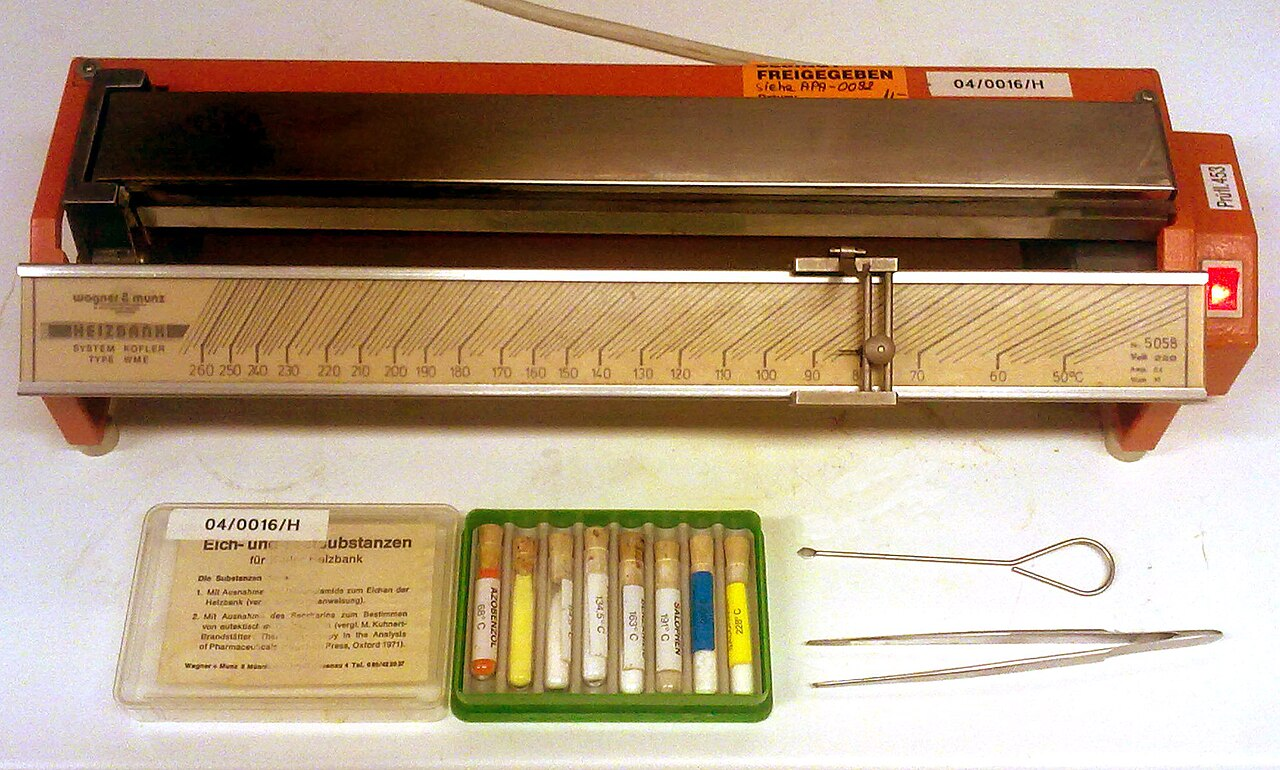
\includegraphics[width=0.62\linewidth]{images/book2/kofler-bench.jpg}

{\small Een verwarmde bank (koflerbank): een metalen strip die aan één
uiteinde verwarmd wordt, met een temperatuurgradiënt over zijn lengte; de
vaste stof, op de strip gestrooid, smelt voorbij een scherpe lijn, die
met de wijzer op de schaal afgelezen wordt. Het doosje bevat
referentiestoffen met een bekend smeltpunt, die dienen om de bank te
kalibreren. Foto: HBR, CC BY-SA 3.0, Wikimedia Commons.}
\end{omfigure}

\begin{method}[Een smeltpunt meten op een verwarmde bank]\label{met:b1:lab-techniques-1:melting-point}
\begin{enumerate}
  \item Zet de bank ruim op voorhand aan: de gradiënt heeft tijd nodig om
        zich in te stellen.
  \item Kalibreer hem met een zuivere referentiestof die dicht bij de
        verwachte waarde smelt, op de strip gestrooid; stel de wijzer zo
        in dat de schaal op de lijn haar smeltpunt aangeeft.
  \item Strooi een paar \omterm{def:b1:crystals-metals:crystal}{kristallen} van het droge monster van het koude
        naar het hete uiteinde; schuif ze met de spatel heen en weer en
        zet de wijzer op de grens waarboven de vaste stof meteen smelt.
  \item Lees af, herhaal, maak de strip schoon; neem het gemiddelde van de
        aflezingen en geef de onzekerheid op
        (\cref{met:b1:lab-techniques-1:report-result}).
\end{enumerate}
\end{method}

Een zuivere kristallijne stof smelt scherp bij haar smeltpunt; een
onzuivere begint lager te smelten en smelt over een temperatuurgebied,
omdat de onzuiverheid de temperatuur verlaagt waarbij de vaste stof en de
vloeistof naast elkaar bestaan (de reden, de chemische potentiaal van een
oplosmiddel die door een opgeloste stof verlaagd wordt, staat in het deel
van jaar 2). Een smeltpunt ver onder de getabelleerde waarde, of een
breed smelttraject, wijst dus op onzuiverheden; een waarde die compatibel
is met de getabelleerde, in de zin van de \omterm{def:b1:lab-techniques-1:z-score}{genormaliseerde afwijking},
ondersteunt de zuiverheid zonder haar te bewijzen.

\begin{inthelab}[De bank kalibreren]
De referenties worden zo gekozen dat ze de verwachte waarde omsluiten.
Aceetanilide, dat bij \qty{114.3}{\celsius} smelt, en benzoëzuur, bij
\qty{122.4}{\celsius}, zijn klassieke standaarden voor producten die
tussen \qty{110}{\celsius} en \qty{130}{\celsius} smelten; voor aspirine
is een standaard dicht bij \qty{135}{\celsius} nog beter. Aspirine zelf
ontleedt bij het smelten, zodat het waargenomen smeltpunt afhangt van hoe
snel ze verwarmd wordt: tabellen geven \qty{135}{\celsius} voor snelle
verwarming, en dat is wat een bank doet.
% ledger: mp:acetanilide, mp:benzoic, mp:aspirin
\end{inthelab}

Een vloeistof wordt geïdentificeerd, en haar zuiverheid gecontroleerd,
aan de hand van haar \emph{brekingsindex} $n_D$, de verhouding van de
lichtsnelheid in vacuüm tot de lichtsnelheid in de vloeistof, gemeten met
de gele D-lijn van natrium bij een opgegeven temperatuur (meestal
\qty{20}{\celsius}), tot op vier decimalen. Water heeft $n_D = 1.333$,
ethanol 1.3611 en cyclohexaan 1.4266 bij \qty{20}{\celsius}. De index
daalt licht als de temperatuur stijgt, daarom wordt het instrument
gethermostatiseerd.
% ledger: nD:water, nD:ethanol, nD:cyclohexane

\begin{omfigure}
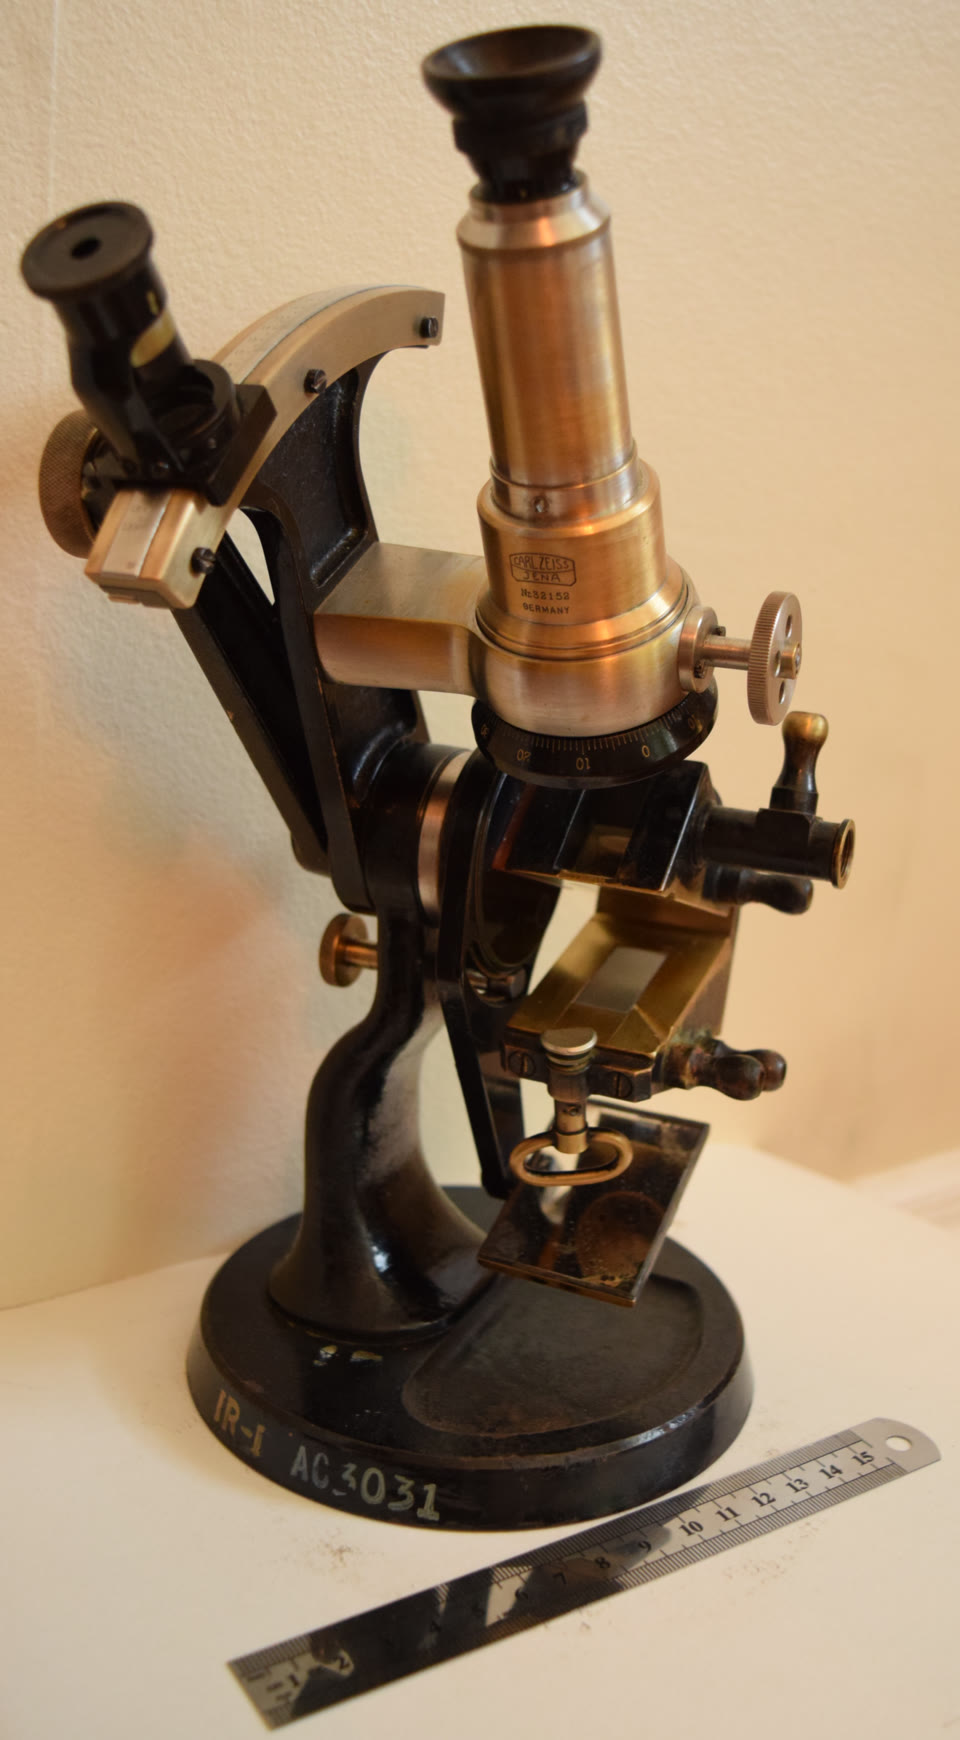
\includegraphics[height=6cm]{images/book2/abbe-refractometer.jpg}

{\small Een abberefractometer: een druppel vloeistof wordt tussen twee
prisma's uitgespreid; het oculair toont een veld dat half licht en half
donker is, en de grens, ingesteld op het dradenkruis, geeft de
brekingsindex op de schaal. Foto: Foreade, CC BY-SA 4.0, Wikimedia
Commons.}
\end{omfigure}

\section{Oefeningen}

\begin{exercise}[$\star$]\label{exo:b1:lab-techniques-1:1}
Een fles propanon draagt de pictogrammen GHS02 en GHS07 en de
aanduidingen H225, H319 en H336. Welk \omterm{def:b1:lab-techniques-1:ghs}{signaalwoord} draagt ze? Welke
aanduidingen beschrijven een fysisch \omterm{def:b1:lab-techniques-1:hazard}{gevaar}, welke een \omterm{def:b1:lab-techniques-1:hazard}{gevaar} voor de
gezondheid? Noem twee voorzorgen die ze vereisen.
\end{exercise}

\begin{exercise}[$\star$]\label{exo:b1:lab-techniques-1:2}
\omterm{def:b1:lab-techniques-1:hazard}{Gevaar} of \omterm{def:b1:lab-techniques-1:hazard}{risico}? (a) Geconcentreerd zwavelzuur veroorzaakt ernstige
brandwonden. (b) \qty{50}{mg} van een giftig poeder afwegen in een
zuurkast met handschoenen stelt de uitvoerder weinig bloot. (c) Natrium
maakt met water waterstof vrij. (d) Hetzelfde oplosmiddel is gevaarlijker
als het heet in een open bekerglas gebruikt wordt dan koud in een
gesloten fles.
\end{exercise}

\begin{exercise}[$\star$]\label{exo:b1:lab-techniques-1:3}
Op een DLC-plaat staat het eluensfront \qty{6.0}{cm} boven de startlijn;
het monster geeft vlekken op \qty{2.1}{cm} en \qty{4.2}{cm}. Bereken hun
$R_f$. Een referentie die op dezelfde plaat aangebracht is, stijgt tot
\qty{4.2}{cm}: wat kan je wel en wat kan je niet besluiten?
\end{exercise}

\begin{exercise}[$\star$]\label{exo:b1:lab-techniques-1:4}
Een buret met een schaalverdeling om de \qty{0.1}{mL} wordt tot op een
half schaaldeel afgelezen. Bereken de \omterm{def:b1:lab-techniques-1:uncertainty}{standaardonzekerheid} van één
aflezing, en daarna van een afgeleverd volume, het verschil van twee
aflezingen.
\end{exercise}

\begin{exercise}[$\star\star$]\label{exo:b1:lab-techniques-1:5}
Vijf wegingen van hetzelfde monster geven \qty{0.2512}{g},
\qty{0.2508}{g}, \qty{0.2515}{g}, \qty{0.2510}{g} en \qty{0.2505}{g}.
Bereken het gemiddelde, de experimentele standaardafwijking en de
\omterm{def:b1:lab-techniques-1:uncertainty}{standaardonzekerheid} van het gemiddelde, en rapporteer het resultaat met
$k = 2$.
\end{exercise}

\begin{exercise}[$\star\star$]\label{exo:b1:lab-techniques-1:6}
Een opgeloste stof met \omterm{def:b1:lab-techniques-1:partition-coefficient}{verdelingscoëfficiënt} $K = 3$ tussen een
organisch oplosmiddel en water wordt uit \qty{50}{mL} water geëxtraheerd
met in totaal \qty{30}{mL} oplosmiddel. Bereken de geëxtraheerde fractie
in één portie, in twee porties van \qty{15}{mL}, en in drie van
\qty{10}{mL}.
\end{exercise}

\begin{exercise}[$\star\star$]\label{exo:b1:lab-techniques-1:7}
Een \omterm{def:b1:titration-methods:titration}{titratie} geeft een concentratie van \qty{0.1012}{mol/L} met een
\omterm{def:b1:lab-techniques-1:uncertainty}{standaardonzekerheid} van \qty{0.0006}{mol/L}; de oplossing werd bereid op
\qty{0.1000}{mol/L} met een \omterm{def:b1:lab-techniques-1:uncertainty}{standaardonzekerheid} van \qty{0.0002}{mol/L}.
Zijn de twee waarden compatibel? En als de onzekerheid van de \omterm{def:b1:titration-methods:titration}{titratie}
\qty{0.0004}{mol/L} was geweest?
\end{exercise}

\begin{exercise}[$\star\star$]\label{exo:b1:lab-techniques-1:8}
De oplosbaarheden (illustratieve waarden, \unit{g} per \qty{100}{mL}) van
een vaste stof in drie oplosmiddelen zijn: oplosmiddel P, 1.5 koud en 2.0
kokend; oplosmiddel Q, 0.3 koud en 12 kokend; oplosmiddel R, 9 koud en 25
kokend. Welk oplosmiddel past bij een \omterm{def:b1:lab-techniques-1:recrystallisation}{herkristallisatie}, en waarom niet de
andere twee? Wat is, met het juiste oplosmiddel, de grootste fractie van
\qty{5.0}{g} van de vaste stof die teruggewonnen kan worden, als het
minimum aan kokend oplosmiddel gebruikt wordt en het mengsel afgekoeld
wordt?
\end{exercise}

\begin{exercise}[$\star\star$]\label{exo:b1:lab-techniques-1:9}
Een kleurloze vloeistof, gethermostatiseerd op \qty{20}{\celsius}, heeft
$n_D = 1.3612$. Welke van water, ethanol en cyclohexaan kan het zijn?
Waarom wordt de temperatuur opgegeven? Wat zou een waarde van 1.350
suggereren?
\end{exercise}

\begin{exercise}[$\star\star\star$]\label{exo:b1:lab-techniques-1:10}
Toon met de gegevens van \cref{exo:b1:lab-techniques-1:6} aan dat, hoe
fijn de \qty{30}{mL} oplosmiddel ook verdeeld wordt, hoogstens een fractie
$1 - \mathrm{e}^{-KV/V_a}$ van de opgeloste stof geëxtraheerd kan worden,
en bereken die. Hoeveel porties bereiken \qty{99}{\percent} van die
limiet?
\end{exercise}

\begin{exercise}[$\star\star\star$]\label{exo:b1:lab-techniques-1:11}
Van een grootheid is bekend dat ze tussen $x_0 - a$ en $x_0 + a$ ligt,
waarbij waarden dicht bij $x_0$ waarschijnlijker zijn: haar dichtheid is
driehoekig, $(a - |x - x_0|)/a^2$. Ga na dat ze genormeerd is en toon aan
dat haar \omterm{def:b1:lab-techniques-1:uncertainty}{standaardonzekerheid} $a/\sqrt6$ is. Vergelijk met het
rechthoekige geval.
\end{exercise}

\begin{exercise}[$\star\star\star$]\label{exo:b1:lab-techniques-1:12}
Een standaardoplossing wordt gemaakt door het monster van
\cref{exo:b1:lab-techniques-1:5} (molaire massa \qty{204.2}{g/mol}, met
verwaarloosbare onzekerheid) op te lossen in een maatkolf van
\qty{100.00}{mL} waarvan het volume een \omterm{def:b1:lab-techniques-1:uncertainty}{standaardonzekerheid} van
\qty{0.06}{mL} heeft. Bereken de concentratie en haar relatieve en
\omterm{def:b1:lab-techniques-1:uncertainty}{uitgebreide onzekerheid}. Welke bron overheerst?
\end{exercise}

\section{Probleem: aspirine zuiveren}

\begin{problem}[{Weekendprobleem --- de gevaren van een synthese, de
herkristallisatie van ruwe aspirine en haar rendement, een smeltpunt met
zijn type-A- en type-B-onzekerheden, en de genormaliseerde afwijking ten
opzichte van de getabelleerde waarde}]
\label{pb:b1:lab-techniques-1:1}
Een student maakt aspirine door \qty{2.00}{g} salicylzuur met een
overmaat ethaanzuuranhydride te verwarmen, en herkristalliseert daarna
het ruwe product. Molaire massa's (\unit{g/mol}): salicylzuur
\ce{C7H6O3} 138.0, aspirine \ce{C9H8O4} 180.0, ethaanzuuranhydride
\ce{C4H6O3} 102.0. Etiketten: salicylzuur GHS05, GHS07, H302, H318;
ethaanzuuranhydride GHS02, GHS05, GHS06, GHS07, H226, H302, H314, H332;
aspirine GHS07, H302. \omterm{def:b1:precipitation:solubility}{Oplosbaarheid} van aspirine in water:
\qty{3.3}{g/L} bij \qty{25}{\celsius}. Getabelleerd smeltpunt van
aspirine (snelle verwarming): \qty{135}{\celsius}.
% ledger: ghs:salicylic, ghs:acetic-anhydride, ghs:aspirin, sol:aspirin-25,
% mp:aspirin, hstat:H318, hstat:H226, hstat:H314, hstat:H302

\medskip
\noindent\textbf{Deel I --- \omterm{def:b1:lab-techniques-1:hazard}{Gevaren}.}
\begin{enumerate}
  \item Wat betekent elk pictogram op het etiket van ethaanzuuranhydride?
  \item Welk \omterm{def:b1:lab-techniques-1:ghs}{signaalwoord} draagt het etiket van salicylzuur? En dat van
        aspirine?
  \item Ethaanzuuranhydride heeft de ernstigste \omterm{def:b1:lab-techniques-1:hazard}{gevaren}. Leg uit hoe het
        \omterm{def:b1:lab-techniques-1:hazard}{risico} van het hanteren van \qty{5}{mL} ervan toch klein gemaakt
        kan worden.
  \item Welke aanduidingen van het anhydride vereisen een veiligheidsbril
        en handschoenen, en welke de zuurkast en de afwezigheid van
        vlammen?
  \item Wat doe je meteen als er een druppel anhydride in een oog komt?
  \item Het filtraat van de \omterm{def:b1:lab-techniques-1:recrystallisation}{herkristallisatie} bevat ethaanzuur en een
        beetje ethanol in water. Waar gaat het naartoe?
\end{enumerate}

\noindent\textbf{Deel II --- Synthese en \omterm{def:b1:lab-techniques-1:recrystallisation}{herkristallisatie}.}
\begin{enumerate}[resume]
  \item Schrijf de vergelijking van de synthese op, met ethaanzuur
        \ce{C2H4O2} als bijproduct, en ga na dat ze kloppend is.
  \item Bereken de hoeveelheid stof salicylzuur en de maximale massa
        aspirine.
  \item Het ruwe droge product weegt \qty{2.41}{g}. Waarom kan de
        \omterm{def:b1:lab-techniques-1:recrystallisation}{herkristallisatie} niet overgeslagen worden, hoewel dat
        \qty{92}{\percent} van het maximum is?
  \item Aspirine wordt geherkristalliseerd uit een beetje ethanol,
        aangevuld met heet water. Waarom is de \omterm{def:b1:precipitation:solubility}{oplosbaarheid} in water bij
        \qty{25}{\celsius}, vergeleken met die dicht bij het kookpunt, de
        eigenschap die ertoe doet?
  \item Waarom wordt de ruwe vaste stof in het minimum aan heet
        oplosmiddel opgelost?
  \item Waarom wordt de oplossing langzaam afgekoeld, en daarna in ijs?
  \item \qty{40}{mL} filtraat bij \qty{25}{\celsius} verlaat de trechter,
        daarna \qty{5}{mL} waswater. Schat de massa aspirine die ermee
        verloren gaat.
  \item Het zuivere droge product weegt \qty{1.95}{g}. Bereken het
        \omterm{def:b1:extent-q-and-k:fractional-extent}{rendement}.
\end{enumerate}

\noindent\textbf{Deel III --- Smeltpunt.}
\begin{enumerate}[resume]
  \item Zes aflezingen op de bank, die net daarvoor gekalibreerd werd,
        geven 134, 135, 133, 135, 134 en \qty{136}{\celsius}. Bereken het
        gemiddelde.
  \item Bereken de experimentele standaardafwijking.
  \item Leid de \omterm{def:b1:lab-techniques-1:uncertainty}{standaardonzekerheid} van type A van het gemiddelde af.
  \item Elke aflezing gebeurt tot op de graad. Bereken de
        afleesonzekerheid van type B.
  \item De kalibratie van de bank is gegarandeerd tot op
        $\pm\qty{1}{\celsius}$. Bereken de overeenkomstige onzekerheid van
        type B, en daarna de gecombineerde \omterm{def:b1:lab-techniques-1:uncertainty}{standaardonzekerheid}.
  \item Rapporteer het smeltpunt met zijn \omterm{def:b1:lab-techniques-1:uncertainty}{uitgebreide onzekerheid}
        ($k = 2$).
  \item Het ruwe product van een klasgenoot smelt tussen 120 en
        \qty{128}{\celsius}. Wat wijst dat aan?
\end{enumerate}

\noindent\textbf{Deel IV --- Vergelijking met de referentie.}
\begin{enumerate}[resume]
  \item De getabelleerde waarde wordt tot op de eenheid gegeven. Welke
        \omterm{def:b1:lab-techniques-1:uncertainty}{standaardonzekerheid} impliceert dat?
  \item Op een DLC-plaat (front \qty{6.0}{cm}) toont het ruwe product
        vlekken op \qty{2.3}{cm} en \qty{3.3}{cm}, salicylzuur één vlek op
        \qty{2.3}{cm}, het geherkristalliseerde product één vlek op
        \qty{3.3}{cm}. Bereken de $R_f$-waarden en besluit.
  \item Waarom hangt het smeltpunt van aspirine af van de
        verwarmingssnelheid?
  \item Bereken de \omterm{def:b1:lab-techniques-1:z-score}{genormaliseerde afwijking} $z$ tussen het gemeten en het
        getabelleerde smeltpunt, en zeg of ze compatibel zijn.
\end{enumerate}
\end{problem}
